\documentclass{article}
\usepackage{polski}
\usepackage[utf8]{inputenc}
\usepackage[top=2cm, bottom=2cm, left=2cm, right=2cm]{geometry}
\usepackage{secdot}
\sectiondot{subsection}
\usepackage{scrextend}
\usepackage{booktabs}
\usepackage{array}
\usepackage{ltablex}
\usepackage{amsmath}
\usepackage{amsfonts}
\usepackage{listings}
\usepackage{parskip}
\addtokomafont{labelinglabel}{\sffamily}
\usepackage{graphicx}
\graphicspath{ {./} }
\lstset{language=Pascal}

\title{\vspace{7cm}\LARGE Analiza algorytmów\\semestr 16Z\\Zadanie 2.}
\author{\LargeŁukasz Wlazły\\nr albumu: 269365}
\date{}

\begin{document}
	\maketitle
	\pagenumbering{gobble}
	\newpage
	\pagenumbering{arabic}

	\section{Treść zadania}

	Nauczycielka w przedszkolu chce rozdać ciastka dzieciom w swojej grupie. Dzieci siedzą w linii obok siebie (i nie zmieniają pozycji). Każde dziecko ma przypisaną ocenę $  s_{i}, i \in (1, 2, \ldots, n) $ zgodnie z~wynikiem testu umiejętności.
	Nauczycielka chce dac każdemu dziecko co najmniej jedno ciastko. Jeśli dzieci siedzą obok siebie, dziecko z wyższą oceną musi dostac więcej ciastek niż to z niższą oceną. Nauczycielka ma ograniczony budżet, więc chce rozdać jak najmniej ciastek. Zaproponuj algorytm, który zwróci najmniejszą liczbę ciastek, które musi rozdać nauczycielka.

	\section{Algorytm}

	\subsection{Założenia}

	\begin{enumerate}
		\item Dziecko, które ma wokół siebie tylko dzieci z wyższymi oceniami, dostaje jedno ciastko.
		\item Jeśli dzieci mają taką samą ocenę i siedzą obok siebie, to dostają tyle samo ciastek.
		\item W poniższych listingach przyjęto, że tablice są indeksowane od 1 do n.
	\end{enumerate}

	\subsection{Rozwiązanie brute force}
		Liczba ciastek, jaką dostanie każde z dzieci, zależy w ogólnym przypadku od ocen wszystkich pozostałych dzieci. Rozwiązanie naiwne polega na ciągłym aktualizowaniu informacji o liczbie ciastek wśród dzieci. W ten sposób po każdym przydzieleniu ciastka i-temu dziecku, liczba ciastek dzieci w~przedziale $[1, i]$ spełnia warunki zadania. Złożoność takiego rozwiązania wynosi $O(n^2)$.
		\begin{lstlisting}[tabsize=2,frame=single]
coockies[1] = 1;

for i = 2 to n do:
	if mark[i] > mark[i-1] then:
	 	coockies[i] = coockies[i-1] + 1;

	if mark[i] == mark[i-1] then:
		coockies[i] = coockies[i - 1];

	if mark[i] < mark[i-1] then:
		coockies[i] = 1;

		for j = i - 1 to 0 do:
			if mark[j] > mark[j+1] AND coockies[j] == coockies[j+1] then:
				coockies[j]++;

			if mark[j] == mark[j+1] then:
				coockies[j] = coockies[j+1];

result = 0;
for i = 1 to n do:
	result += coockies[i];

return result;
		\end{lstlisting}
	\newpage
	\subsection{Rozwiązanie optymalne}
		W tym podejściu liczbę ciastek i-tego dziecka rozważamy jako maksimum iteracji lewo- i prawostronnej. Jeśli, idąc z lewej strony, zawsze przydzielamy minimalną liczbę ciastek, a następnie zrobimy to samo idąc z~prawej strony, to finalnie maksimum z tych dwóch przebiegów będzie minimalną liczbą ciastek, jaką powinno dostać dziecko. Złożoność tego rozwiązania wynosi $O(n)$.
		\begin{lstlisting}[tabsize=2, frame=single]
coockies[i] = 1;
result = 0;

for i = 2 to n do:
	if mark[i] > mark[i-1] then:
		coockies[i] = coockies[i-1] + 1;

	if mark[i] == mark[i-1] then:
		coockies[i] coockies[i-1];

	if mark[i] < mark[i-1] then:
		coockies[i] = 1;

for i = n-1 to 1 do:
	if mark[i] > mark[i+1] then:
		coockies[i] = max(coockies[i+1] + 1, coockies[i]);

	if mark[i] == mark[i+1] then:
		coockies[i] = coockies[i+1];

	result += coockies[i];

result += coockies[n];

return result;

		\end{lstlisting}

	\subsection{Złożoność pamięciowa}
	Przyjmując, że ocena jednego ucznia oraz ilość ciastek, jaką dostaje, zajmują jedną komórkę pamięci, algorytm posiada złożoność pamięciową określoną wzorem:
	\begin{align*}
		M(n) = 2n
	\end{align*}

	\subsection{Złożoność czasowa}
	Operacją podstawową algorytmu jest wykonanie obliczeń na pojedynczej komórce ciągu wejściowego lub pomocniczego. Wobec tego złożoność czasowa wynosi:
	\begin{align*}
		T(n) = 2n
	\end{align*}

	\newpage
	\section{Przypadki trywialne}

	\subsection{Ciąg stały}

	Jeśli wszystkie dzieci otrzymały taką samą ocenę, to wynikiem działania algorytmu jest:
	\begin{align*}
		n
	\end{align*}

	\subsection{Ciąg malejący lub rosnący}

	Jeśli oceny dzieci układają się w ciąg rosnący lub malejący, to wynikiem działania algorytmu jest:
	\begin{align*}
		\displaystyle\sum_{i=1}^{n} i
	\end{align*}

	\section{Porównanie złożoności teoretycznej z eksperymentalną}
	W celu porównania zależności posłużono się zależnością:
	\begin{align*}
		q(n) = \frac{t(n)}{cT(n)}
	\end{align*}
	gdzie $t(n)$ to rzeczywisty czas obliczeń, $T(n)$ to wartość teoretyczna, a $c$ stała wyliczona na podstawie mediany. \\
	W tym przypadku:
	\begin{align*}
		c = \frac{261}{4000} = 0,06525
	\end{align*}

	\begin{center}
		\begin{tabular}{l l l}
			\toprule
				$n$ & $t(n) [\mu s]$ & $q(n) $\\
			\midrule
				10 & 9 & 13,8 \\
				100 & 29 & 4,44 \\
				500 & 85 & 2,61 \\
				1000 & 87 & 1,33 \\
			\midrule
				4000 & 261 & 1,0 \\
			\midrule
				8000 & 513 & 0,98 \\
				20000 & 1474 & 1,13 \\
				40000 & 2498 & 0,96 \\
				100000 & 7412 & 1,16 \\
			\bottomrule
		\end{tabular}
	\end{center}

	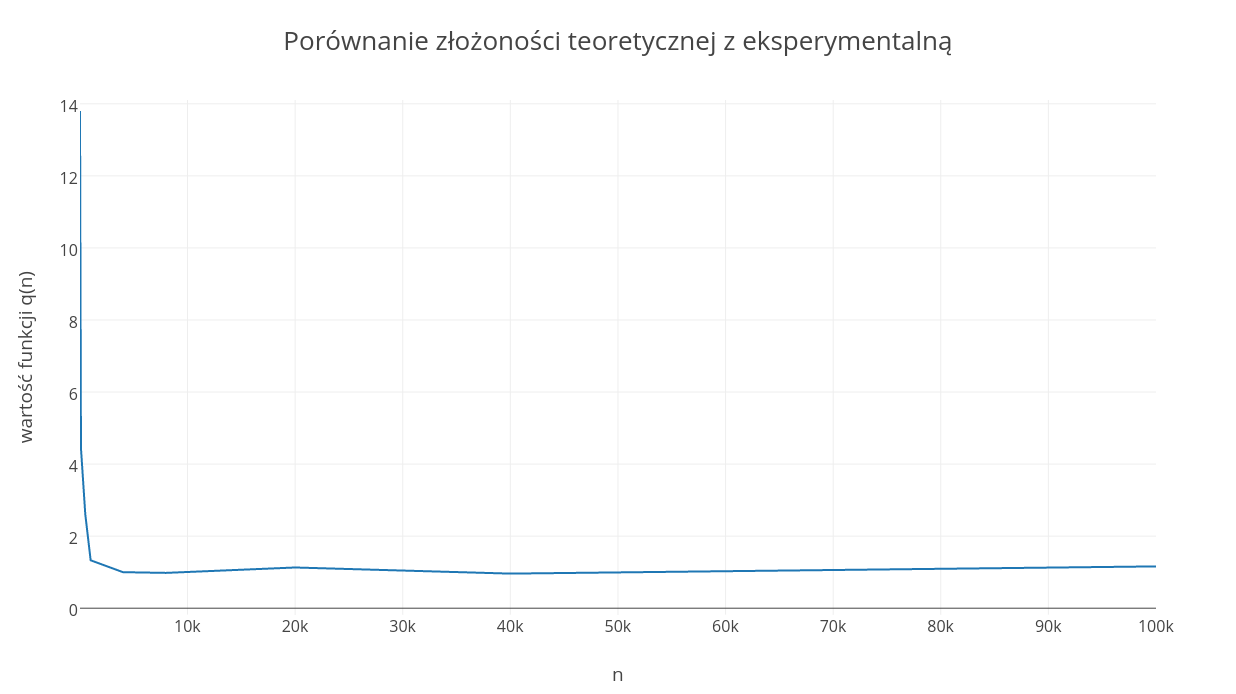
\includegraphics[width=\textwidth]{plot.png}

\end{document}
